%
% 卒論レジュメフォーマット Ver.2.0 pLaTeX版
%
\documentclass[twocolumn]{jarticle} % 2段組のスタイルを用いている

\usepackage{wuse_resume}
\usepackage{url}	% \url{}コマンド用.URLを表示する際に便利
\usepackage{float}
%\usepackage[dvipdfmx]{graphicx}  % ←graphicx.styを用いてEPSを取り込む場合有効にする
			% 他のパッケージ・スタイルを使う場合には適宜追加

\usepackage{otf}
\usepackage{xcolor}
\usepackage[dvipdfmx]{graphicx}
\usepackage{float}
%\usepackage{graphicx}  % ←graphicx.styを用いてEPSを取り込む場合有効にする
			% 他のパッケージ・スタイルを使う場合には適宜追加

\newcommand{\RQOne}{Good First Issue に貢献している開発者のうち,新参開発者の割合はどの程度か}
\newcommand{\RQTwo}{熟練者は新参開発者をどの程度待っているか}
\newcommand{\RQThree}{ゲーム理論に基づくと,熟練者はどの程度の期間新参開発者のために GFI の解決を待つのが適切か}

\newcommand{\NIssue}{180,671}
\newcommand{\NTrueIssue}{17,956}
\newcommand{\NGFI}{478}
\newcommand{\NNormal}{17,478}
\newcommand{\NBOT}{5}

%%%%%%%%%%%%%%%%%%%%%%%%%%%%%%%%%%%%%%%%%%%%%%%%%%%%%%%%%%%%%%%%%%%%%%%%

%%
%% タイトル,学生番号,氏名などを設定する
%%

\タイトル{新参開発者向けの障害対応のジレンマ\\〜熟練者が介入するタイミングの分析〜}
\研究室{ソーシャルソフトウェア工学}
\学生番号{60246191}
\氏名{中井 大雄}

\概要{%
本研究では,オープンソースソフトウェア(OSS)開発において,新参開発者の課題解決を熟練者がどれだけ待っているかを実証データとゲーム理論で得られる解を比較し,分析する.OSSプロジェクトは新参開発者を獲得するために,新参者が取り組みやすい課題に「Good First Issue(GFI)」ラベルを付与している.しかし,先行研究\cite{GFI}では熟練開発者がGFIを解決する事例が多いと指摘されている.本研究では,GFIに取り組む開発者の経験値を調査し,GFIが新参者に活用されているかを検証する.また,熟練者はどの程度の期間GFIを代行して解決するのを待っているかを調査し,介入時期をゲーム理論で分析する. 
}

\キーワード{オープンソースソフトウェア}
\キーワード{GitHub}
\キーワード{オンボーディング}
\キーワード{Good First Issue}
\キーワード{ゲーム理論}

%%%%%%%%%%%%%%%%%%%%%%%%%%%%%%%%%%%%%%%%%%%%%%%%%%%%%%%%%%%%%%%%%%%%%%%%

%% 以下の3行は変更しない

\begin{document}
\maketitle
\thispagestyle{empty} % タイトルを出力したページにもページ番号を付けない

%%%%%%%%%%%%%%%%%%%%%%%%%%%%%%%%%%%%%%%%%%%%%%%%%%%%%%%%%%%%%%%%%%%%%%%%

%%
%% 本文 - ここから
%%

%%%%%%%%%%%%%%%%%%%%%%%%%%%%%%%%%%%%%%%%%%
% 1章 はじめに
\section{はじめに}\label{sec:intro}
%%%%%%%%%%%%%%%%%%%%%%%%%%%%%%%%%%%%%%%%%%

OSSプロジェクトはボランティア開発者によって支えられており,安定した開発体制を維持するためには新参開発者の参加を促すことが重要である.そのため,メンタリング制度\cite{menter1}やポータルサイト\cite{portal}などを活用し,新参開発者の参入障壁を下げる取り組みが行われている.特にGitHubでは,新参開発者向けに「Good First Issue(GFI)」というラベルを付与することで,貢献しやすいIssueを明示している.しかし,先行研究\cite{GFI}では,GFIが経験豊富な開発者によって解決されるケースが指摘されており,その原因として適切でないIssueにGFIラベルが付与されていることが挙げられている.また,新参開発者が現れずにGFIが長期間放置される場合,熟練者が解決せざるを得ず,結果的に新参開発者の参入機会が失われる可能性がある.熟練者は介入のタイミングにジレンマを抱えており,本研究ではその適切なタイミングを明らかにすることを目的とする.

本研究では,3つのResearch Questions(RQ)を設定し,開発者がGFIに介入する際のジレンマについて分析する.

\begin{itemize}
\item RQ1:\RQOne
\item RQ2:\RQTwo
\item RQ3:\RQThree
\end{itemize}

%%%%%%%%%%%%%%%%%%%%%%%%%%%%%%%%%%%%%%%%%%
% 2章 データセット
\section{データセット}\label{sec:rq1}
%%%%%%%%%%%%%%%%%%%%%%%%%%%%%%%%%%%%%%%%%%

GitHub上でGood First Issueを運用しており十分なデータが得られるプロジェクトとして,今回はmicrosoftのvscodeプロジェクトを対象とした.データ収集期間はvscodeプロジェクトが作成された2015年9月3日から2025年1月28日までとした.\NTrueIssue 件のIssueを取得し,GFI \NGFI 件,通常Issueは \NNormal 件に分類した.

%%%%%%%%%%%%%%%%%%%%%%%%%%%%%%%%%%%%%%%%%%
% 3章 RQ1
\section{RQ1:\RQOne}\label{sec:rq1}
%%%%%%%%%%%%%%%%%%%%%%%%%%%%%%%%%%%%%%%%%%

\subsection{手法}
リポジトリのすべてのIssueについて解決者の経験値を取得し,GFIと通常Issueでは貢献した開発者の経験値分布にどのような違いがみられるかを箱ひげ図で比較する.また,2つの分布に有意な差がみられるかをマンホイットニーのU検定を用いて分析する.

\subsection{結果}
結果を図1に示す.GFIと通常Issueに有意差はないと帰無仮説を立てたとき,マンホイットニーのU検定を行うとp値は0.00000であった.また,効果量は-0.668であった.このことから,2つの分布に有意な差があるといえる.

%-------------------
\begin{figure}[H]
\centerline{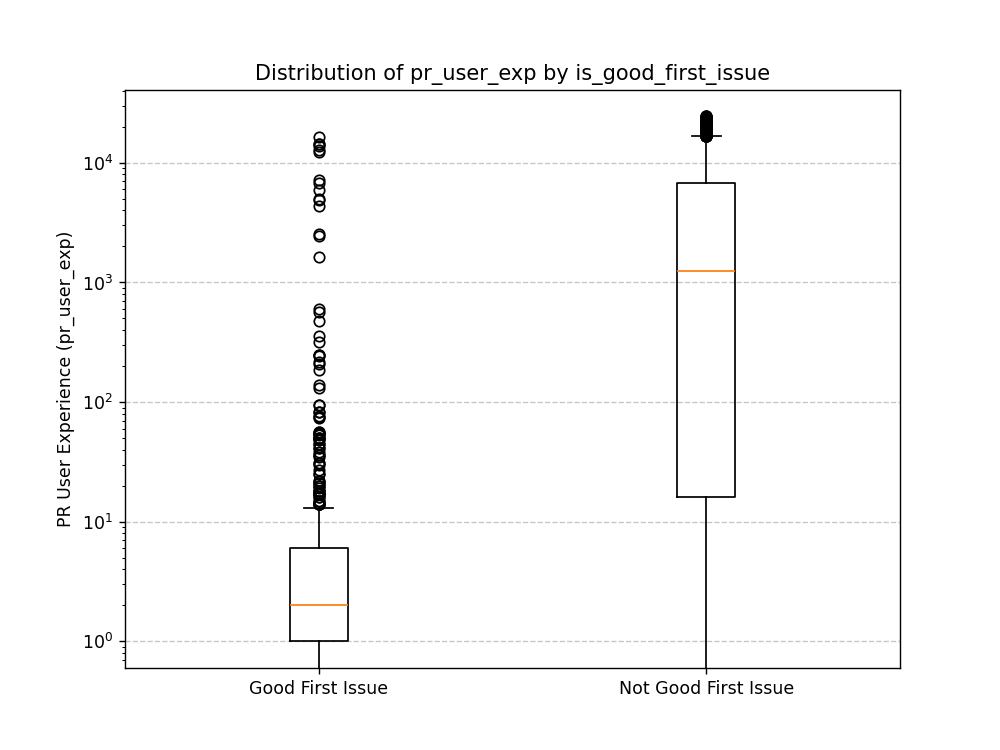
\includegraphics[width=0.9\linewidth]{@BSthesis2024_Nakai/BSthesis2024_Nakai_fig/2025-02-03_11h12_00.png}}
\caption{経験値の箱ひげ図}
\label{fig:milestone}
\end{figure}
%-------------------

%%%%%%%%%%%%%%%%%%%%%%%%%%%%%%%%%%%%%%%%%%
% 4章 RQ2
\section{RQ2:\RQTwo}\label{sec:rq2}
%%%%%%%%%%%%%%%%%%%%%%%%%%%%%%%%%%%%%%%%%%

\subsection{手法}
RQ1と同様のデータセットを用いて,Issueの開放期間とIssueを解決した開発者の経験値の関係を散布図で表現し,GFIと通常Issueでどのような違いがみられるかを分析する.

\subsection{結果}
結果を図2に示す.

%-------------------
\begin{figure}[H]
\centerline{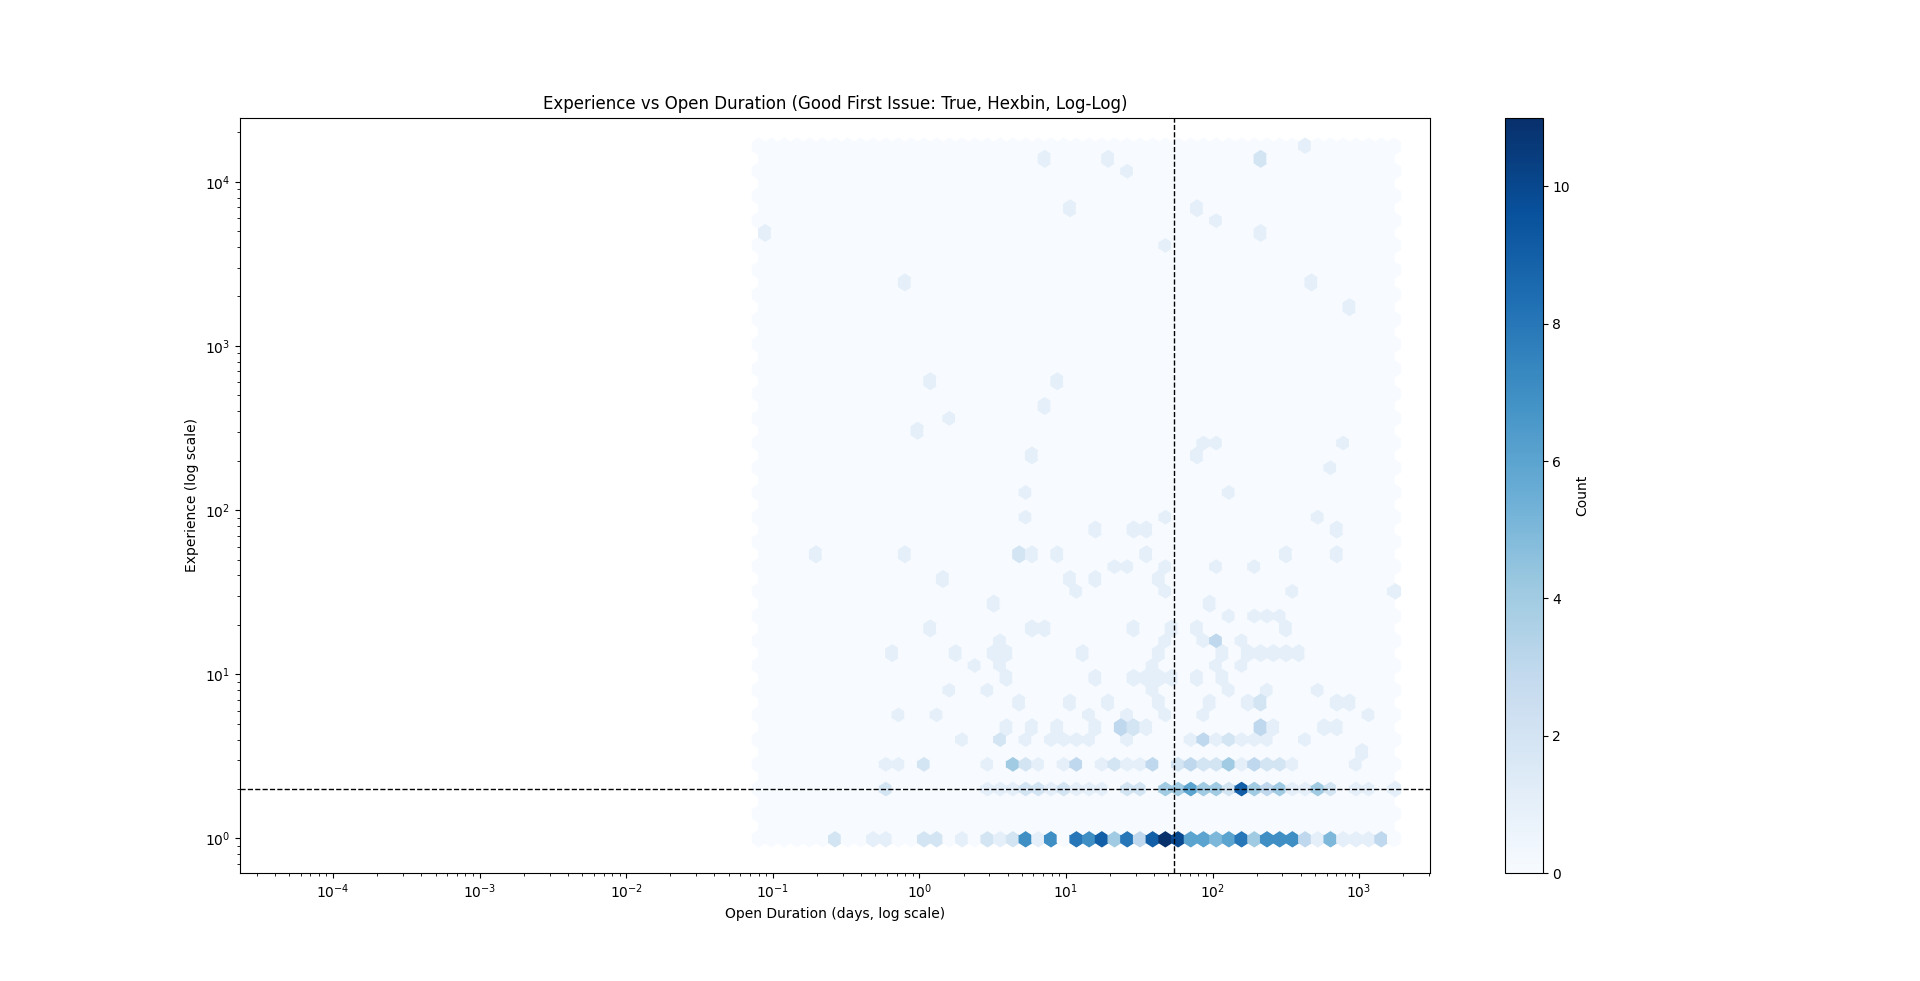
\includegraphics[width=0.9\linewidth]{@BSthesis2024_Nakai/BSthesis2024_Nakai_fig/fhex_blue.png}}
\caption{Issueの開放期間とIssueを解決した開発者の経験値の散布図(GFI)}
\label{fig:milestone}
\end{figure}
%-------------------

%-------------------
\begin{figure}[H]
\centerline{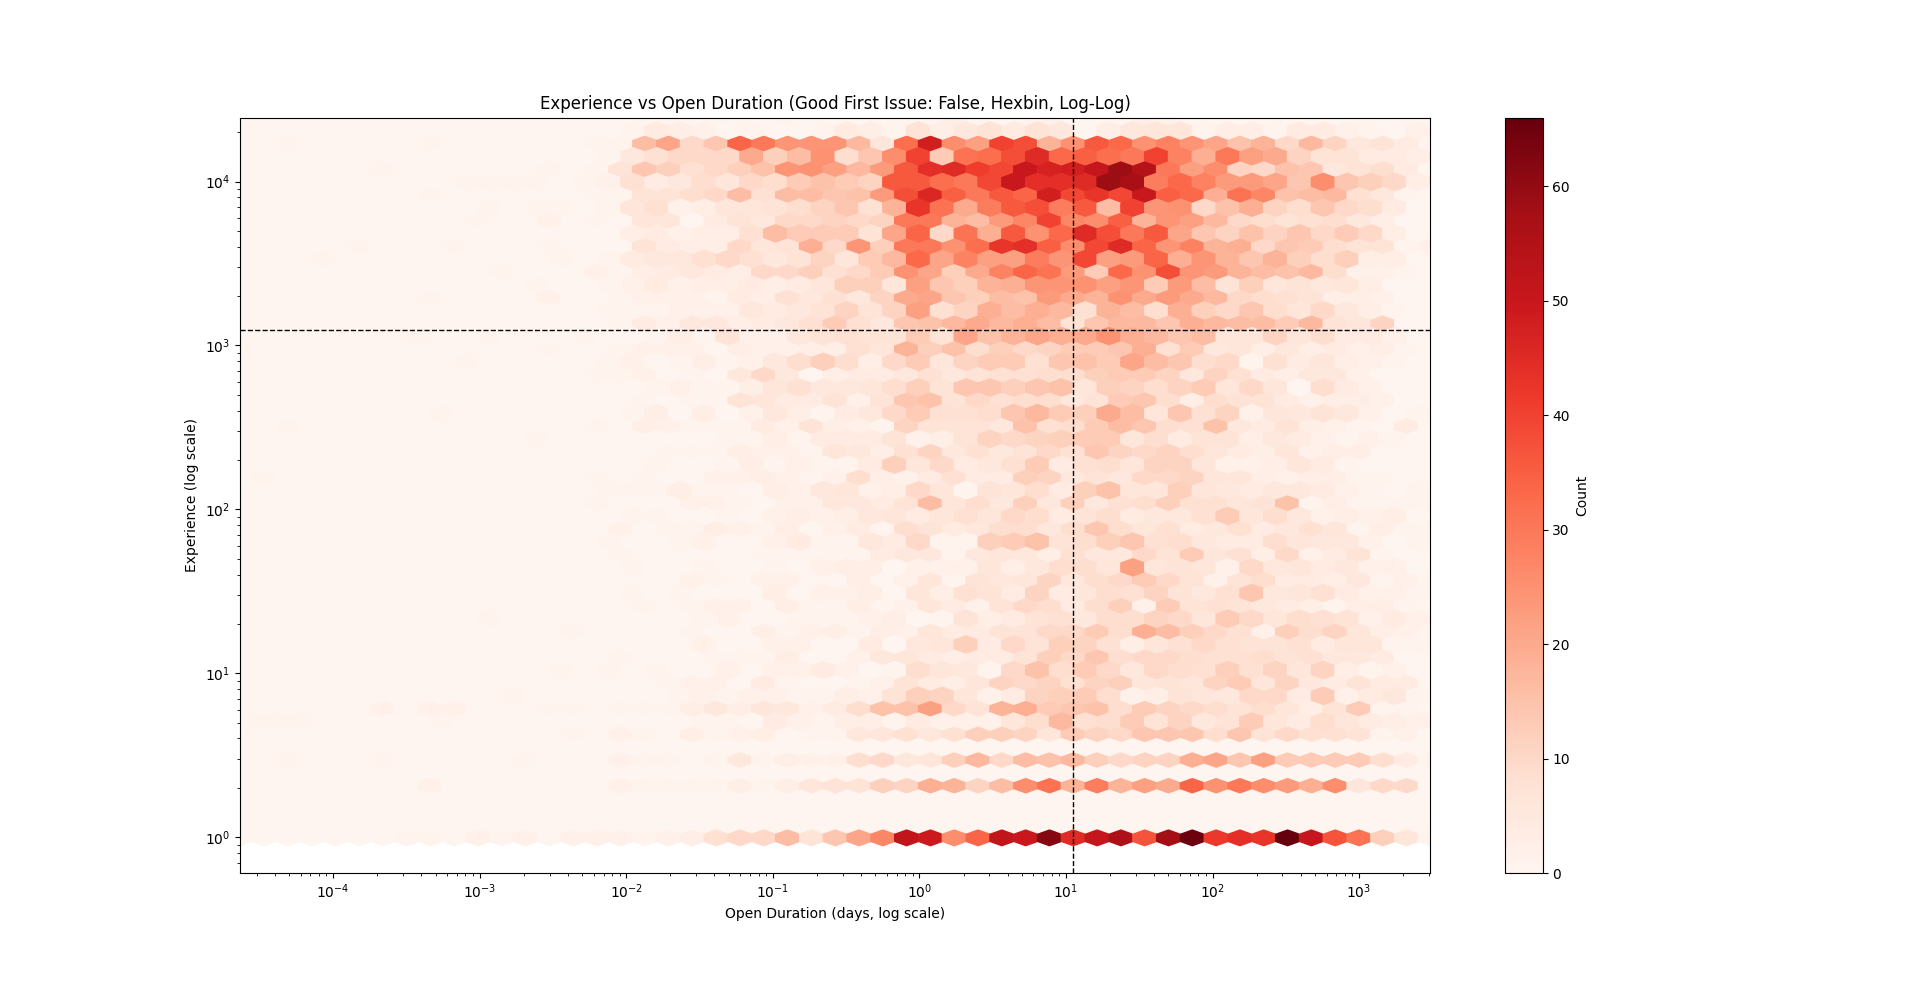
\includegraphics[width=0.9\linewidth]{@BSthesis2024_Nakai/BSthesis2024_Nakai_fig/fhex_red.png}}
\caption{Issueの開放期間とIssueを解決した開発者の経験値の散布図(通常Issue)}
\label{fig:milestone}
\end{figure}
%-------------------

%%%%%%%%%%%%%%%%%%%%%%%%%%%%%%%%%%%%%%%%%%
% 5章 RQ3
\section{RQ3:\RQThree}\label{sec:rq3}
%%%%%%%%%%%%%%%%%%%%%%%%%%%%%%%%%%%%%%%%%%

\subsection{手法}
ゲーム理論を用いて新参開発者,熟練者の貢献へのジレンマを定式化する.

\subsection{結果}
%-------------------
\begin{figure}[H]
\centerline{
\includegraphics[width=0.9\linewidth]{@BSthesis2024_Nakai/BSthesis2024_Nakai_fig/ritoku.png}}
\caption{新参開発者A,熟練者Bの戦略と効用}
\label{fig:milestone}
\end{figure}
%-------------------

期待効用値について考える.Aが貢献する確率を$p$, Bが貢献する確率を$q$とすると,両者の得る期待効用値は以下のように計算できる.

\textbf{新参開発者Aの期待効用値}

$U_A = p(V_A -c_A) + (1 - p)V_Aq + 0*(1-p)(1-q)$

\textbf{熟練者Bの期待効用値}

$U_B = q(V_B -c_B) + (1 - q)V_Ap + 0*(1-p)(1-q)$
\\
$U_A =U_B$となるような均衡条件で解くと,p, qの均衡戦略を求めることができる.

%%%%%%%%%%%%%%%%%%%%%%%%%%%%%%%%%%%%%%%%%%
% 6章 おわりに
\section{おわりに}\label{sec:conclusion}
%%%%%%%%%%%%%%%%%%%%%%%%%%%%%%%%%%%%%%%%%%

本研究では,オープンソースソフトウェア(OSS)開発において,新参開発者の課題解決を熟練者がどれだけ待っているかを分析するため,3つのRQを設定して調査を行った.

RQ1では多くのGFIが新参開発者によって解決される一方で,熟練者によってGFIが解決されるケースも見られた.新参貢献者が貢献を申し出るまでの期間が長く,熟練者がこれを待ちきれなかったことが原因だと考えた.

RQ2では,貢献までの期間が通常Issueに比べてGFIのほうが長いことが分かった.これは,通常Issueの中に早期解決が容易なものが多く含まれていたことが原因だと考えた.また,新参開発者に注目すると通常IssueよりもGFIのほうが解決に時間を要していることも分かった.新参開発者どうしの譲り合いがこのような状況を引き起こすのではないかと考えた.

RQ3ではゲーム理論を用いた分析で熟練者が抱える介入へのジレンマを定式化し,熟練者が解決するGFIの解決までの期間にばらつきがある理由を明らかにした.

%%%%%%%%%%%%%%%%%%%%%%%%%%%%%%%%%%%%%%%%%%%%%%%%%%%%%%%%%%%%%%%%%%%%%%%%

%%
%% 本文 - ここまで
%%

%%%%%%%%%%%%%%%%%%%%%%%%%%%%%%%%%%%%%%%%%%%%%%%%%%%%%%%%%%%%%%%%%%%%%%%%

%%
%% 参考文献
%%

\begin{thebibliography}{99}

\bibitem{GFI}
    堀口 日向. OSSプロジェクトへのオンボーディング支援のためのGood First Issue自動分類 2022.

\bibitem{menter1}
Fabian Fagerholm, Alejandro Guinea, Jay Borenstein, and J¨urgen M¨unch. Onboarding in
Open Source Projects. IEEE Software, Vol. 31, No. 6, pp. 54–61, 2014.

\bibitem{portal}
 Igor Steinmacher, Tayana Uchoa Conte, Christoph Treude, and Marco Aur´elio Gerosa.
Overcoming Open Source Project Entry Barriers with a Portal for Newcomers. In In
Proceedings of the 38th International Conference on Software Engineering (ICSE 2016),
pp. 273–284, 2016.

\end{thebibliography}

%%%%%%%%%%%%%%%%%%%%%%%%%%%%%%%%%%%%%%%%%%%%%%%%%%%%%%%%%%%%%%%%%%%%%%%%

\end{document}